\subsection{Протокол Деннинга~---~Сакко}\index{протокол!Деннинга~---~Сакко|(}
\selectlanguage{russian}

Протокол был предложен в 1981 году сотрудниками Университета Пердью Дороти Деннинг и Джованни Марией Сакко (\langen{Dorothy E. Denning, Giovanni Maria Sacco},~\cite{Denning:Sacco:1981}). В данном протоколе к доверенному центру (Тренту) за сертификатами сразу обоих участников обращается инициатор (Алиса, рис.~\ref{fig:denning-sacco}). Этот же участник отвечает и за формирование нового сессионного ключа $K$.

\begin{figure}
    \centering
    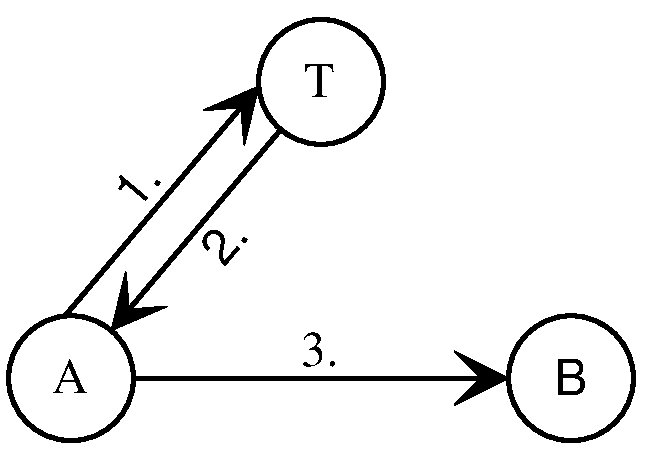
\includegraphics[width=0.5\textwidth]{pic/denning-sacco}
    \caption{Взаимодействие участников в протоколе Деннинга~---~Сакко\label{fig:denning-sacco}}
\end{figure}

\begin{protocol}
    \item[(1)] $Alice \to \left\{ A, B \right\} \to Trent$
    \item[(2)] $Trent \to \left\{ S_T( A, K_A, T_T ), S_T( B, K_B, T_T ) \right\} \to Alice$
	\item[(3)] Алиса генерирует новый сессионный ключ $K$
	\item[{}] $\begin{array}{lll}
Alice \to \{ & E_B( S_A ( K, T_A ) ), & \\ 
             & S_T( A, K_A, T_T ),    & \\ 
             & S_T( B, K_B, T_T )     & \} \to Bob
\end{array}$
	\item[(4)] Боб проверяет подпись доверенного центра на сертификате $S_T( A, K_A, T_T )$, расшифровывает сессионный ключ $K$ и проверяет подпись Алисы.
\end{protocol}

Отсутствие в сообщении $E_B( S_A ( K, T_A ) )$ каких-либо идентификаторов делает протокол уязвимым к атаке с известными сеансовым ключом\index{атака!с известным разовым ключом} и позволяет второй стороне (Бобу) выдать себя за инициатора (Алису) в сеансе с третьей стороной (Кларой, рис.~\ref{fig:denning-sacco-attack}).

\begin{figure}
    \centering
    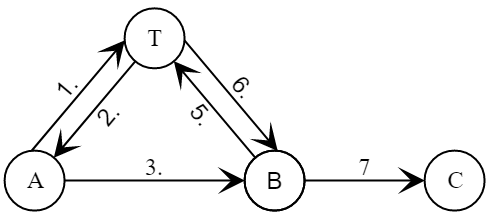
\includegraphics[width=0.67\textwidth]{pic/denning-sacco-attack}
    \caption{Взаимодействие участников в протоколе Деннинга~---~Сакко при атаке с известным разовым ключом\label{fig:denning-sacco-attack}}
\end{figure}

\begin{protocol}
    \item[(1)--(4)] Алиса и Боб провели сеанс протокола, выработав новый сессионный ключ $K$.
    \item[(5)] $Bob \to \left\{ B, C \right\} \to Trent$
    \item[(6)] $Trent \to \left\{ S_T( B, K_B, T_T ), S_T( C, K_C, T_T ) \right\} \to Bob$
	\item[(7)] Боб воспроизводит сообщения $S_A ( K, T_A )$ и $S_T( A, K_A, T_T )$ от Алисы в сеансе с Кларой:
    \item[{}] $\begin{array}{lll}
Bob~(Alice) \to \{ & E_C( S_A ( K, T_A ) ), & \\ 
             & S_T( A, K_A, T_T ),    & \\ 
             & S_T( C, K_C, T_T )     & \} \to Clara
\end{array}$
	\item[(8)] Клара успешно проверяет подпись доверенного центра на сертификате $S_T( A, K_A, T_T )$, расшифровывает сессионный ключ $K$ и проверяет подпись Алисы.
\end{protocol}

В результате Клара уверена, что получила от Алисы новый сессионный ключ $K$.

\index{протокол!Деннинга~---~Сакко|)}